The SPIKE distance proposed by Kreuz et al in \cite{Kreuzetal2011} is an instantaneous parameter-free distance measure between spike-trains.  By instantaneous measure, it is meant that for each time $t$ there is a time-local distance between two spike-trains.  This measure can the be integrated over the length of the spike-trains to give a parameter-free distance measure between spike trains. In the study of spike-train metrics, often a multi-unit measure is desired (to minimise compounding any errors that may result from inefficient spike-sorting?). A multi-unit measure is a distance between collections of labelled spike-trains.  The SPIKE distance in \cite{Kreuzetal2011} does not lend itself to a simple multi-unit extension, so instead a simpler version of the SPIKE distance is extended.

\section{Single-unit recordings}
With a view to extending the SPIKE distance to a multi-unit distance measure, it is useful to review the definition of the SPIKE measure provided in \cite{Kreuzetal2011}:  Given two spike-trains $x$ and $y$, where $x = \{ t_1^x, \ldots, t_n^x \}$ and $y = \{ t_1^y, \ldots , t_m^y\}$, where $t_1^x,\ldots,t_n^x,t_1^y,\ldots,t_m^y$ are the spike times.  The SPIKE distance in \cite{Kreuzetal2011} has the nice property that the distance is bounded such that it is always between zero and one.  Unfortunately, to achieve a "natural" extension to a multi-unit measure, this property is sacrificed.  A simpler version of the distance, without the strict upper bound of one, is used.

The simpler distance is very quick and easy to calculate.  A `gap' is associated with each spike; this is the distance to the nearest spike in the other spike-train.  The total distance between two spike trains is then the sum of these gaps.  The original SPIKE distance included additional normalisation factors that have been omitted in simplifying the measure.  To form the time-local distance, a weighted sum of the gaps for the corner spikes is made, that is, the spikes preceding and following the time of interest in each of the two spike trains.  The weighting is chosen so that the integral of the time-local function is just the sum of the gaps.

First, the gaps are calculated for each spike in the two spike-trains.  This is simply the nearest spike in the other spike train:
\begin{equation}
\Delta t_i^x = min_i ( | t_i^x - t_i^y |)
\end{equation}
At each time instant, these is a unique set of four corner spikes: the preceding and following spikes from each spike train, which are labelled $t_P^x(t), t_F^x(t), t_P^y(t)$ and  $t_F^y(t)$; these are, respectively, the preceding and following spikes in spike-train $x$ and the preceding and following spikes in spike-train $y$.

For each spike-train, w, a time-local distance is then calculated using the associated gap of the four corner spikes for each spike-train, $w=x,y$:
\begin{equation}
s_w(t) = \frac{\lambda_P(t) \Delta t_P^w(t) + \lambda_F(t)\Delta t_F^w(t)}{I^w(t)}
\end{equation}
where
\begin{equation}
\lambda_F^w(t) = \frac{t- t_P^w(t)}{I^w(t)}, \, \lambda_P^w(t) = \frac{ t_F^w(t) - t}{I^w(t)}
\end{equation}
and $I^w(t)$ is the size of the interval in which $t$ is contained:
\begin{equation}
I^w(t) = t_F^w(t) - t_P^w(t).
\end{equation}
Now, the time-local distance for each neuron is added to give the overall time-local distance:
\begin{equation}
s(t) = s_x(t) + s_y(t).
\end{equation}

This simplified time-local SPIKE distance has the advantage that its integral is simply the sum of the gaps of each spike; that is:
\begin{equation}
\int_0^T s(t)\, dt = \sum_w \sum_i \Delta t_i^w.
\end{equation}

In practice this simplified version of SPIKE produces similar time profiles to the version described in \cite{Kreuzetal2011}. The time-local distance profile for two similar spike-trains is given in Figure [NEED TO ADD PICTURE].

\section{Extension to multi-unit recordings}

In the multi-unit case a distance is defined between two multi-unit recordings.  Thus, rather than two spike-trains there are two sets of spike-trains; $\mathbf{X}=\{ \mathbf{x}_i \}$ and $ \mathbf{Y}=\{ \mathbf{y}_i \}$, where $i \in 1\ldots N$ and the index $i$ labels the neuron.

Here the single-unit distance above is extended to a multi-unit distance by including the possibility that the nearest spike for one neuron may belong to a different neuron in the other set, however there is a distance penalty associated with changing from one neuron to the other. This penalty is similar to the ``costs'' in edit-length metrics such as Victor-Purpura \cite{VictorPurpura1997}. In other words, it is necessary to introduce a parameter $k$, which quantifies a fictional distance between spikes fired in different cells.  The size of this distance quantifies the importance of the labelling of the neurons, and varying $k$ interpolates smoothly from $k=0$, a summed population (SP) code, to $k$ large, a labeled line  (LL) code.  While theoretically the LL code occurs as $k \rightarrow \infty$, in practice a LL code occurs when $k$ is on the order of $2/\lambda$, where $\lambda$ is the average frequency of the trials.   The gaps can then be calculated as follows:

\begin{equation}
\Delta t_{\alpha}^{\mathbf{x}_i} = \min_{\beta,j} \left( |t_{\alpha}^{\mathbf{x}_i} - t_{\beta}^{\mathbf{y}_j} | + k\left[1-\delta(i,j)\right] \right)
\end{equation}
where $\delta(i,j)$ is the Kroneker delta. Hence, if the spikes have the same label in $\mathbf{x}$ and $\mathbf{y}$ there is no added distance, otherwise $k$ is added to the time difference between the spikes.  This is illustrated in Figure \ref{fig:gaps2}:

\begin{figure}[Thb]
\begin{center}
\setlength{\unitlength}{.1cm}
\begin{picture}(100,40)

\linethickness{1.5pt}
\put(5,8.7){\mbox{$\mathbf{2}$}}
\put(5,28.7){\mbox{$\mathbf{1}$}}
\put(10,10){\line(1,0){80}}
\put(10,30){\line(1,0){80}}

\linethickness{1pt}
\put(85,20){\vector(0,1){10}}
\put(85,20){\vector(0,-1){10}}
\put(87,18.5){\mbox{$k$}}

\put(20,11){\line(0,1){2}}
\put(20,12){\line(1,0){5}}
\put(25,12){\vector(0,1){16}}

\put(25,31){\line(0,1){2}}
\put(30,32){\vector(1,0){10}}
\put(30,32){\vector(-1,0){5}}
\put(40,31){\line(0,1){2}}

\put(50,11){\line(0,1){2}}
\put(55,12){\vector(1,0){5}}
\put(55,12){\vector(-1,0){5}}
\put(60,11){\line(0,1){2}}

\put(65,31){\line(0,1){2}}
\put(70,32){\vector(1,0){5}}
\put(70,32){\vector(-1,0){5}}
\put(75,31){\line(0,1){2}}

\put(18.5,9.1){\mbox{$\times$}}
\put(58.5,9.1){\mbox{$\times$}}
\put(63.5,29.1){\mbox{$\times$}}
\put(38.5,29.1){\mbox{$\times$}}
\put(25,30){\circle{2}}
\put(50,10){\circle{2}}
\put(75,30){\circle{2}}
\end{picture}
\end{center}
\caption{\label{fig:gaps2}An example of how to calculate the gaps between spikes.  If  the circles represent spikes from $\mathbf{X}$ and crosses represent spikes from $\mathbf{Y}$, then in the picture above, the distance $k$ is simply the cost of relabelling a spike.  We also see that the gaps are not necessarily symmetric.}

\end{figure}






The time-local distance measure is then defined as before, using the corner spikes normalised by the inter-spike-interval:
\begin{equation}
s_{\mathbf{X}}(t) = \sum_{\mathbf{x}_i \in \mathbf{X}} \frac{\lambda_{\mathrm{P}}(t)\Delta t_{\mathrm{P}}^{\mathbf{x}_i} (t) + \lambda_{\mathrm{F}}(t)\Delta t_{\mathrm{F}}^{\mathbf{x}_i}(t) }{I^{\mathbf{x}_i}(t) }%t_{\mathrm{F}}^{\mathbf{x}_i} - t_{\mathrm{P}}^{\mathbf{x}_i}}
\end{equation}
where 
\begin{equation}
\lambda_{\mathrm{F}}^{\mathbf{x}_i}(t) =\frac{ t-t_{\mathrm{P}}^{\mathbf{x}_i}(t)}{I^{\mathbf{x}_i}(t)}%t_{\mathrm{F}}^{\mathbf{x}_i}(t) - t_{\mathrm{P}}^{\mathbf{x}_i}(t)}
\end{equation}
and
\begin{equation}
 \lambda_{\mathrm{P}}^{\mathbf{x}_i}(t) =\frac{ t_{\mathrm{F}}^{\mathbf{x}_i}(t) - t}{I^{\mathbf{x}_i}(t)}%{t_{\mathrm{F}}^\mathbf{x}_i}(t) - t_{\mathrm{P}}^{\mathbf{x}_i}(t)}
\end{equation}
and $I^{\mathbf{x}_i}(t)$ is the length of the interval in the spike-train $\mathbf{x}_i$ containing $t$, $I^{\mathbf{x}_i}(t) = t_{\mathrm{F}}^{\mathbf{x}_i}(t) - t_{\mathrm{P}}^{\mathbf{x}_i}(t)$.
 As before:
\begin{equation}
s(t) = s_{\mathbf{X}}(t) + s_{\mathbf{Y}}(t)
\end{equation}

Once more, this distance measure has the nice property that if the time-local measure is integrated over the course of the trial it equals the sum of the gaps of each spike:
\begin{equation}
\int_0^T s(t)\,dt = \sum_{\mathbf{W}} \sum_{\mathbf{w}_i \in \mathbf{W}} \sum_{\alpha} \Delta t_{\alpha}^{\mathbf{w}_i}
\end{equation}
\bigskip
%
%\begin{figure}[hbt]
%\include{spikemaxvmin}
%\caption{Performance of the proposed distance measure for different values of the mixing parameter $a$.  For each value of the mixing parameter $a$ the average value of the Transmitted Information is calculated for different values of $k$.  The solid line shows the maximum value over $k$, and the dotted line is the minimum value.  This figure should be compared to Figure 3 in \cite{HoughtonSen2008}.\label{fig:spikeminmax} }
%\end{figure}

 \subsection{Testing on data}
% 
% \begin{figure}[thb]
%\include{spikebest}
%\caption{The relationship between $k$ and $a$.  For each value of $a$, the value of $k$ giving the highest Transmitted Information is calculated over 20 runs.  The average is plotted, along with error bars representing the standard deviation.\label{fig:bestk}}
%\end{figure}

 The multi-unit distance measure was tested on similar test data to that found in Houghton \& Sen \cite{HoughtonSen2008}, where two Poisson neurons form a receptive field and are each connected to two leaky integrate-and-fire neurons with relative strength $a$ and $1-a$.  Hence, for $a=0$ each receptive neuron is connected to a single LIF neuron, and for $a=0.5$, each LIF neuron receives input equally from each of the receptive neurons.  
%
%\begin{figure}[htb]
%\include{spikeratio}
%\caption{The ratio of the transmitted information, $h$ of a labelled-line code (LL) and a summed-population code (SP).  For LL, $h$ is calculated for $k$ large, and for SP, $h$ is calculated for $k=0$. \label{fig:ratio}}
%\end{figure}
%\section{}
%\subsection{}
\newpage
\section{ISI distance}
\bigskip
\subsection{Single unit recordings}

With a view to extending the ISI distance to a multi-unit distance measure, it is useful to review the previous definition of the ISI distance between two spike trains $\mathbf{x}$ and $\mathbf{y}$ .  The ISI distance can be thought of as a rate-comparison, where the inter-spike interval (ISI) is used as a proxy for the firing rate.  As with all the time-local distance measures, it is defined as the interval over time of a local distance function $s(t)$.

Given two spike-trains $\mathbf{x}$ and $\mathbf{y}$, then $I^{\mathbf{x}}(t)$, $I^{\mathbf{y}}(t)$ are the inter-spike intervals at time $t$, for the spike-trains $\mathbf{x}$ and $\mathbf{y}$.  The time-local distance function is then defined in Kreuz et al. (2007) as:
\begin{equation}
s(t) = \left\{ \begin{array}{ll} 1-I^{\mathbf{x}}(t) / I^{\mathbf{y}}(t)  & \text{if } I^{\mathbf{x}}(t) \leq I^{\mathbf{y}}(t) \\ 1- I^{\mathbf{y}}(t) / I^{\mathbf{x}}(t)  & \text{otherwise} \end{array} \right.
\end{equation}
From the point of view of generalising to more than one neuron, it is convenient to rewrite this as:
\begin{equation}
s(t) = \frac{ | I^{\mathbf{x}}(t) - I^{\mathbf{y}}(t) | }{\max (I^{\mathbf{x}}(t), I^{\mathbf{y}}(t)) }
\end{equation}

\subsection{Initial extension to multi-unit recordings}

In the multi-unit case a distance is defined to be between two multi-unit recordings.  Thus, rather than two spike-trains there are two sets of spike-trains; $\mathbf{X}=\{ \mathbf{x}_i \}$ and $ \mathbf{Y}=\{ \mathbf{y}_i \}$, where $i \in 1\ldots N$ and the index $i$ is labelling the neuron.

The ISI-distance is a rate-based metric, so here a similar approach to multi-unit recordings as was used successfully for the van Rossum metric, another metric calculated using estimated rates, is used.  That approach, outlined in Houghton and Sen (2008) \cite{HoughtonSen2008}, replaces the rate with a rate-vector in an $N$-dimensional space.  To do this, each neuron is assigned a unit vector describing its direction in the rate-space.  At a given time, this is multiplied by the estimated rate of the neuron to give a rate-vector. The population rate-vector is then the sum of individual rate-vectors for each of the neurons in the population.  

An $L^1$ norm, $| I^{\mathbf{x}}(t) - I^{\mathbf{y}}(t) | $, appears in the numerator of $s(t)$ in the single-unit case, so the natural extension of this idea to the multi-unit ISI-distance involves an $L^1$-structure on the $N$-dimensional space, which is the ISI-space in this case. In practice this means the individual vectors are unit vectors under the $L^1$-norm; so for example for $N=2$, one vector may be $(1,0)$ and the other one would be $(1-\alpha,\alpha)$.  The corresponding individual neuron ISI-vectors would then be: 
\begin{equation}
\mathbf{I}^{\mathbf{x}_1}(t)=\begin{pmatrix}I^{\mathbf{x}_1}(t)\\0\end{pmatrix}
\end{equation}
\begin{equation}
\mathbf{I}^{\mathbf{x}_2}(t) = \begin{pmatrix} (1-\alpha)I^{\mathbf{x}_2}(t)\\ \alpha I^{\mathbf{x}_2}(t)\end{pmatrix}.
\end{equation}
The overall population ISI-vector $\mathbf{I^x}(t) = \mathbf{I}^{\mathbf{x}_1}(t) + \mathbf{I}^{\mathbf{x}_2}(t)$:
\begin{equation}
\mathbf{I^X}(t) = \begin{pmatrix} I^{\mathbf{x}_1}(t) + I^{\mathbf{x}_2}(t) - \alpha I^{\mathbf{x}_2}(t) \\ \alpha I^{\mathbf{x}_2}(t) \end{pmatrix}
\end{equation}

It remains to extend the definition of $s(t)$ to ISI-vectors. It is proposed here that this should be:
\begin{equation}
s(t) = \frac{ \| \mathbf{I^X}(t) - \mathbf{I^Y}(t) \|_1 }{ \sum_i \max ( I^X_i, I^Y_i ) }
\end{equation}
where $I^X_i, \, I^Y_i$ are the $i$th components of $\mathbf{I^X}$ and $\mathbf{I^Y}$ respectively, and:
\begin{equation}
\| \mathbf{I^X}(t) - \mathbf{I^Y}(t) \|_1 = \sum_i | I^X_i - I^Y_i |
\end{equation}

One important property of any multi-unit distance measure is that it interpolates from the summed population (SP) code  to the labelled line (LL) code .  In the case of the labelled line code, it is necessary to consider what the result should be, for example in the Victor Purpura metric the LL code is the sum of the distances of the individual neurons, whereas in the case of the van Rossum metric, the LL code is the Pythagorean sum of the distances.  Here the LL code corresponds to when the vectors are all perpendicular,   this is $\alpha=1$ in the $N=2$ example above.  Up to an overall $L^1$ rotation, this means that the individual ISI vectors will have a single non-zero component, and $s(t)$ is given by:
\begin{equation}
s(t) = \frac{\sum_i | I^{\mathbf{x}_i} (t)  - I^{\mathbf{y}_i}(t)|}{\sum_i \max (I^{\mathbf{x}_i},I^{\mathbf{y}_i})}
 \end{equation}
 Given the rational structure of the ISI-distance, this seems to be the natural structure for the LL code.  
Conversely, when all the vectors are parallel, the result is the SP code:
\begin{equation}
s(t) = \frac{| \sum_i I^{\mathbf{x}_i}(t) - \sum_i I^{\mathbf{y}_i}(t) |}{\max (\sum_i I^{\mathbf{x}_i}(t),\sum_i I^{\mathbf{y}_i}(t) )}
\end{equation}
in which, effectively, the ISIs are averaged across the population before being compared in the distance measure.
%
%\begin{figure}[bht]
%\begin{center}
%% GNUPLOT: LaTeX picture with Postscript
\begingroup
  \makeatletter
  \providecommand\color[2][]{%
    \GenericError{(gnuplot) \space\space\space\@spaces}{%
      Package color not loaded in conjunction with
      terminal option `colourtext'%
    }{See the gnuplot documentation for explanation.%
    }{Either use 'blacktext' in gnuplot or load the package
      color.sty in LaTeX.}%
    \renewcommand\color[2][]{}%
  }%
  \providecommand\includegraphics[2][]{%
    \GenericError{(gnuplot) \space\space\space\@spaces}{%
      Package graphicx or graphics not loaded%
    }{See the gnuplot documentation for explanation.%
    }{The gnuplot epslatex terminal needs graphicx.sty or graphics.sty.}%
    \renewcommand\includegraphics[2][]{}%
  }%
  \providecommand\rotatebox[2]{#2}%
  \@ifundefined{ifGPcolor}{%
    \newif\ifGPcolor
    \GPcolorfalse
  }{}%
  \@ifundefined{ifGPblacktext}{%
    \newif\ifGPblacktext
    \GPblacktexttrue
  }{}%
  % define a \g@addto@macro without @ in the name:
  \let\gplgaddtomacro\g@addto@macro
  % define empty templates for all commands taking text:
  \gdef\gplbacktext{}%
  \gdef\gplfronttext{}%
  \makeatother
  \ifGPblacktext
    % no textcolor at all
    \def\colorrgb#1{}%
    \def\colorgray#1{}%
  \else
    % gray or color?
    \ifGPcolor
      \def\colorrgb#1{\color[rgb]{#1}}%
      \def\colorgray#1{\color[gray]{#1}}%
      \expandafter\def\csname LTw\endcsname{\color{white}}%
      \expandafter\def\csname LTb\endcsname{\color{black}}%
      \expandafter\def\csname LTa\endcsname{\color{black}}%
      \expandafter\def\csname LT0\endcsname{\color[rgb]{1,0,0}}%
      \expandafter\def\csname LT1\endcsname{\color[rgb]{0,1,0}}%
      \expandafter\def\csname LT2\endcsname{\color[rgb]{0,0,1}}%
      \expandafter\def\csname LT3\endcsname{\color[rgb]{1,0,1}}%
      \expandafter\def\csname LT4\endcsname{\color[rgb]{0,1,1}}%
      \expandafter\def\csname LT5\endcsname{\color[rgb]{1,1,0}}%
      \expandafter\def\csname LT6\endcsname{\color[rgb]{0,0,0}}%
      \expandafter\def\csname LT7\endcsname{\color[rgb]{1,0.3,0}}%
      \expandafter\def\csname LT8\endcsname{\color[rgb]{0.5,0.5,0.5}}%
    \else
      % gray
      \def\colorrgb#1{\color{black}}%
      \def\colorgray#1{\color[gray]{#1}}%
      \expandafter\def\csname LTw\endcsname{\color{white}}%
      \expandafter\def\csname LTb\endcsname{\color{black}}%
      \expandafter\def\csname LTa\endcsname{\color{black}}%
      \expandafter\def\csname LT0\endcsname{\color{black}}%
      \expandafter\def\csname LT1\endcsname{\color{black}}%
      \expandafter\def\csname LT2\endcsname{\color{black}}%
      \expandafter\def\csname LT3\endcsname{\color{black}}%
      \expandafter\def\csname LT4\endcsname{\color{black}}%
      \expandafter\def\csname LT5\endcsname{\color{black}}%
      \expandafter\def\csname LT6\endcsname{\color{black}}%
      \expandafter\def\csname LT7\endcsname{\color{black}}%
      \expandafter\def\csname LT8\endcsname{\color{black}}%
    \fi
  \fi
  \setlength{\unitlength}{0.0500bp}%
  \begin{picture}(7200.00,5040.00)%
    \gplgaddtomacro\gplbacktext{%
      \csname LTb\endcsname%
      \put(1078,767){\makebox(0,0)[r]{\strut{} 0}}%
      \put(1078,1356){\makebox(0,0)[r]{\strut{} 0.25}}%
      \put(1078,1946){\makebox(0,0)[r]{\strut{} 0.5}}%
      \put(1078,2535){\makebox(0,0)[r]{\strut{} 0.75}}%
      \put(1078,3125){\makebox(0,0)[r]{\strut{} 1}}%
      \put(1078,3714){\makebox(0,0)[r]{\strut{} 1.25}}%
      \put(1078,4303){\makebox(0,0)[r]{\strut{} 1.5}}%
      \put(1210,484){\makebox(0,0){\strut{} 0}}%
      \put(2329,484){\makebox(0,0){\strut{} 0.1}}%
      \put(3447,484){\makebox(0,0){\strut{} 0.2}}%
      \put(4566,484){\makebox(0,0){\strut{} 0.3}}%
      \put(5684,484){\makebox(0,0){\strut{} 0.4}}%
      \put(6803,484){\makebox(0,0){\strut{} 0.5}}%
      \put(176,2771){\rotatebox{-270}{\makebox(0,0){\strut{}h}}}%
      \put(4006,154){\makebox(0,0){\strut{}alpha}}%
    }%
    \gplgaddtomacro\gplfronttext{%
    }%
    \gplbacktext
    \put(0,0){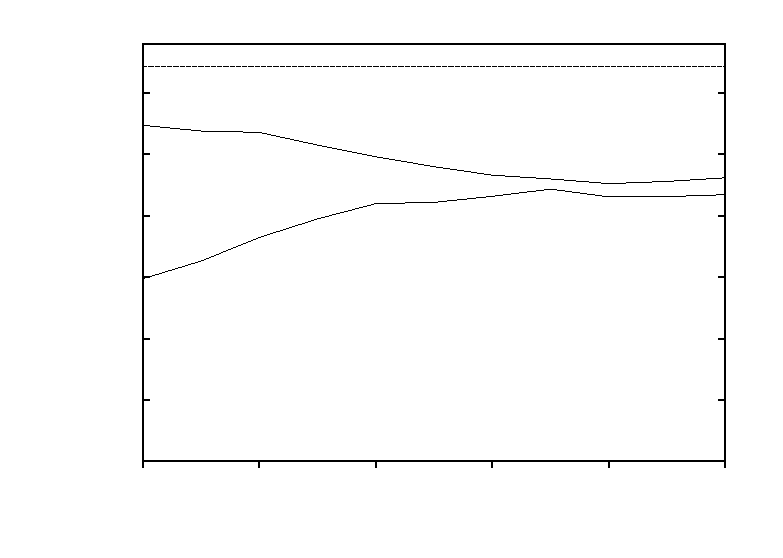
\includegraphics{maxmin}}%
    \gplfronttext
  \end{picture}%
\endgroup

%\end{center}
%\caption{Performance of the metric for different values of the mixing parameter $a$.  For each value of the mixing parameter $a$ the average value of the Transmitted Information is calculated for different values of $\alpha$.  The solid line shows the maximum value over $\alpha$, and the dotted line is the minimum value.  This figure should be compared to Figure 3 in \cite{HoughtonSen2008}.\label{fig:minmax}}
%\end{figure}

\subsection{Numerical tests}
This multi-unit extension of the ISI distance is tested on the same data that was used to test the multi-unit van Rossum distance in Houghton and Sen (2006).   In this simulation, two integrate and fire neurons receive noisy input from two sources.  A parameter $a$ determines how much these two inputs are mixed.  If $a=0$ each receives independent input, if $a=0.5$, each receives an input averaging the two sources.  Both neurons also receive shot noise.  The two inputs are inhomogeneous Poisson processes, and there are five separate randomly chosen inhomogeneous functions. Each of these are used to drive the neurons 20 times, and the distance function is used to cluster these 100 neurons by stimulus in the usual way.  The accuracy of this clustering is evaluated by calculating the Transmitted Information ($h$) of the clustering.  The results are shown in Figures \ref{fig:minmax} and \ref{fig:bestalpha} . Compared to similar graphs in \cite{HoughtonSen2008}, the performance is similar to the multi-unit van Rossum metric; but compared to the van Rossum metric, the optimal value of $\alpha$ in the distance measure is less clearly modulated by $a$.  

%
%\begin{figure}[thb]
%\begin{center}
%\include{best}
%\end{center}
%\caption{ The relationship between $\alpha$ and $a$.  For each value of $a$, the value of $\alpha$ giving the highest Transmitted Information is calculated over 20 runs.  The average is plotted, along with error bars representing the standard deviation.\label{fig:bestalpha} }
%\end{figure}

While the extension proposed above was derived logically from the single-unit case, it does not agree with the standard definition of a summed-population code, that is, it is possible to find a population of neurons which have spiked at exactly the same time, but where the average inter-spike intervals are not equal at a moment in time.

\subsection{Alternative extensions to the multi-unit case}

Upon comparing the above extension to the previous extension to the multi-unit case by Kreuz et al. \cite{Kreuzetal2009}, it became clear that there was a fundamental difference in how each distance measure viewed the concept of a rate-based metric.


The extension proposed in \cite{Kreuzetal2009} interpolates between the average of the individual ISI distances and the ISI distance of the two ``population neurons'', that is, treating the individual spike times from the entire population as though they were all from the same neuron.  This is done with a ``population parameter'' $p$, which runs from $0$ (SP) to $1$ (LL).  This is given by:
\begin{equation}
\label{pop}
s(t) = (1-p)\left( \frac{ | I^{\mathbf{x}}(t) - I^{\mathbf{y}}(t) |}{ \max (I^{\mathbf{x}},I^{\mathbf{y}})}\right) + p\left( \frac{\sum_i | I^{\mathbf{x}_i}(t) - I^{\mathbf{y}_i}(t) |}{\sum_i \max (I^{\mathbf{x}_i},I^{\mathbf{y}_i})} \right),
\end{equation}
with notation as before, and $I^{\mathbf{x}}(t)$ is the interval in $\mathbf{x}$ at time $t$, where the population is viewed as a single neuron.

%\begin{figure}[thb]
%\begin{center}
%\input{popmaxvmin}
%\end{center}
%\caption{\label{popmaxmin}This is the performance of the extension proposed in the paper by Kreuz et al. \cite{Kreuzetal2009}.  The solid line represents the average of the maximum transmitted information ($h$) value across 20 trials, and the dotted line the minimum.  As we saw with the previous metric, the more the inputs are mixed, the more difficult it is to cluster the responses.}
%\end{figure}

The extension proposed above can be compared to the Kreuz extension by replacing the ISI of the ``population neuron'' with the average of the ISIs across the population of neurons.  This leads to the following equation: 
\begin{equation}
\label{av}
s(t) = (1-p) \left(\frac{ | \sum_i I^{\mathbf{x}_i}(t) - \sum_i I^{\mathbf{y}_i}(t) |}{\max (\sum_i I^{\mathbf{x}_i}(t),\sum_i I^{\mathbf{y}_i}(t) )}\right) + p\left( \frac{\sum_i | I^{\mathbf{x}_i}(t) - I^{\mathbf{y}_i}(t) |}{\sum_i \max (I^{\mathbf{x}_i},I^{\mathbf{y}_i})} \right),
\end{equation}.


%\begin{figure}[htb]
%\begin{center}
%\include{newmaxvmin}
%\end{center}
%\caption{\label{avmaxmin} This is the performance of the alternative extension, using the average ISI, proposed here as a complementary measure. The solid line again represents the average of the maximum transmitted information across 20 trials, and the dotted lie the minimum.  The maximum is very comparable to the population ISI measure. The average ISI's minimum transmitted information performs worse when the signals are separate, and considerably better when the signals are mixed.}
%\end{figure}

There is a fundamental difference in how each of these distance measures view what a SP metric should be.  The Kreuz example believes that there is information being carried by the frequency of arrival of spikes across the population, regardless of origin, and the second measure using the average ISI believes that each neuron is essentially carrying the same message, with an inherent noise due to the biological constraints of neurons.  Each argument has its own merits {\bf[I think we should find a few papers where each side of the argument would be given merit by the results]}, and it could be useful to have both of these measures, as in equations \ref{pop} and \ref{av}, depending on the focus of the experiment.

{\bf [combine the population distance and the average distance graphs into one graph]}

\newpage
\section{Adaptive SPIKE \& ISI distances}

The downside to the measures introduced above is that there must be parameters to vary between the SP and LL cases, and there is no good way to choose a parameter, which often leads to a grid search to find the optimal parameter.  A goal of this work is to find a way for the data itself to choose its own population parameter.  The SPIKE and ISI distances for single neurons are both parameter-free, so it would be ideal if an extension could be found that was also parameter-free.

Since the ISI distance is a distance based on the firing rate of the neurons, the assumption was made that if the rates of the individual neurons were reasonably similar throughout the two populations, then the correct code to use would be an SP code, whereas if they were very different, then a LL code should be used.

The ISI extensions above have a population parameter $p$ that varies from $0$ to $1$, so a measure of similarity (or dissimilarity) that varies from 0 to 1 would be ideal.  The normalised cross-entropy of the ISIs of the two populations is such a measure.  Labelling the ISIs as above, the cross-entropy at any point in time $t$ is calculated as:
\begin{equation}
h_{\mathbf{X}, \mathbf{Y}}(t) = \frac{1}{\log 2n}\sum_{\mathbf{z}\in\mathbf{x,y}}\sum_i -\frac{I^{z_i}(t)}{\sum_{\mathbf{z}}\sum_i I^{z_i}(t)} \log\left(\frac{I^{z_i}(t)}{\sum_{\mathbf{z}}\sum_i I^{z_i}(t)}\right)
\end{equation}

This is a dissimilarity measure on the ISIs across the two populations.  If the ISIs are very similar, then the cross-entropy is close to 1, if they are very dissimilar then it is close to 0.  Thus, the cross-entropy is a good candidate for an instantaneous population parameter $p$, or more accurately $(1-p)$.

Figures \ref{adpop} and \ref{adav} show that this does not work very well, because one would hope that the adaptive measure would perform on a par with the maximum values of transmitted information from figures \ref{popmaxmin} and \ref{avmaxmin}, but it is considerably lower than the max values in both the "average" and "population" ISI measures.


%\begin{figure}[Bht]
%\begin{center}
%\include{adaptivepop}
%\end{center}
%\caption{\label{adpop}Using the same tests as before, the transmitted information of the "average" ISI distance using the cross-entropy to get our population parameter $p$.}
%\end{figure}
%
%\begin{figure}[Bht]
%\begin{center}
%\include{adaptiveav}
%\end{center}
%\caption{\label{adav}Using the same tests as before, the transmitted information of the "average" ISI distance using the cross-entropy to get our population parameter $p$.}
%\end{figure}
